\section{Datengrundlage}

\subsection{Sensoraufbau und Ansichten}

Die Szene wird von zwei Ouster-LiDAR-Sensoren mit einer Aufnahmerate von ungefähr 10\,Hz erfasst. Jeder Sensor besitzt zunächst ein eigenes Koordinatensystem. Aus den Rohdaten werden drei Eingabevarianten erzeugt:

\begin{itemize}
    \item \texttt{os0}: transformierte Punktwolke des ersten Sensors,
    \item \texttt{os1}: transformierte Punktwolke des zweiten Sensors,
    \item \texttt{merged}: geometrisch registrierte und zusammengefügte Punktwolke beider Sensoren.
\end{itemize}

Eine Einzelsensor-Punktwolke enthält typischerweise ungefähr 105.000 Punkte, die fusionierte Punktwolke ungefähr 210.000 Punkte. Abbildung~\ref{fig:setup} zeigt den Grundriss des Versuchsbereichs mit den Sensorpositionen.

\begin{figure}[H]
\centering
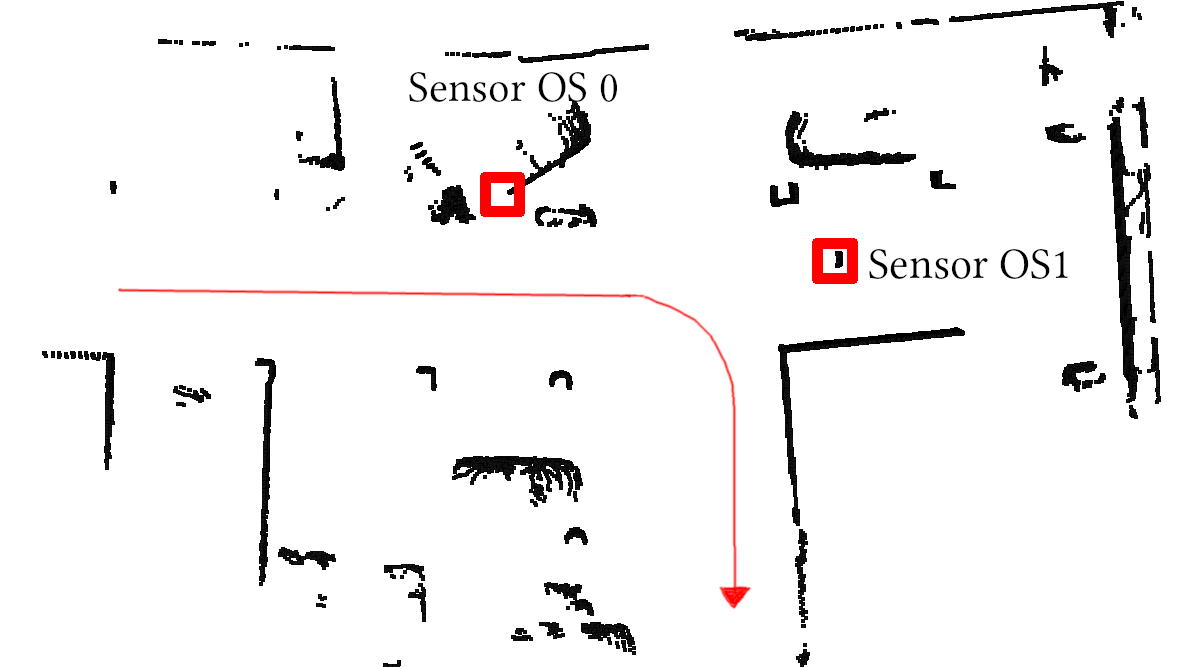
\includegraphics[width=0.85\textwidth]{images/Setup.png}
\caption{Grundriss des Versuchsbereichs in der Tiefgarage des Fraunhofer FOKUS mit den Sensorpositionen OS0 und OS1 entlang der markierten Route. Aus \cite[Abb.~21]{pagel2025railway}.}
\label{fig:setup}
\end{figure}

Die Fusion erhöht damit die Punktdichte und ergänzt verdeckte Objektseiten, vergrößert aber zugleich die zu verarbeitende Datenmenge und den sichtbaren Hintergrund.

\subsection{Aufgezeichnete Experimente}

Am 9. Oktober 2025 wurden neun Bewegungsaufnahmen in derselben Tiefgaragenszene erstellt (Tabelle~\ref{tab:experiments}):

\begin{table}[H]
\centering
\begin{tabular}{cc}
\toprule
\textbf{Experimente} & \textbf{Bewegte Zielklasse} \\
\midrule
1--3 & Auto \\
4--6 & Fahrrad \\
7--9 & Person \\
\bottomrule
\end{tabular}
\caption{Aufgezeichnete Experimente und die jeweils bewegte Zielklasse.}
\label{tab:experiments}
\end{table}

Neben dem jeweiligen bewegten Zielobjekt enthält die Szene zahlreiche statische Objekte, insbesondere geparkte Fahrzeuge. Diese statischen Objekte sind für eine realistische Detektion relevant, dürfen bei der Interpretation der Generalisierungsleistung aber nicht mit vollständig neuen Objektinstanzen verwechselt werden: Sie stehen über viele Aufnahmen hinweg an denselben Positionen.

Für die abschließende Cross-Validation wird ausschließlich die Schnittmenge der gültigen Zeitstempel aller drei Ansichten verwendet. Dadurch erhält jede Ansicht dieselben 2.122 physischen Frames. Die Annotationen bleiben dennoch ansichtsspezifisch, weil ein Objekt je nach Sensorabdeckung und Sichtbarkeit nicht in jeder Ansicht in exakt denselben Frames annotiert ist.

\subsection{Annotationen}

Die Ground-Truth-Annotationen bestehen aus orientierten dreidimensionalen Bounding Boxes. Für jede Box werden Klasse, Position, Abmessungen und Orientierung gespeichert. Zusätzlich kennzeichnet ein \texttt{static}-Attribut statische Objekte. Die finalen Labels wurden mit dem projektspezifischen Editor \texttt{experiment/manual\_bbox\_editor.py} geprüft und korrigiert (Abbildung~\ref{fig:manual-labeling}).

\begin{figure}[H]
\centering
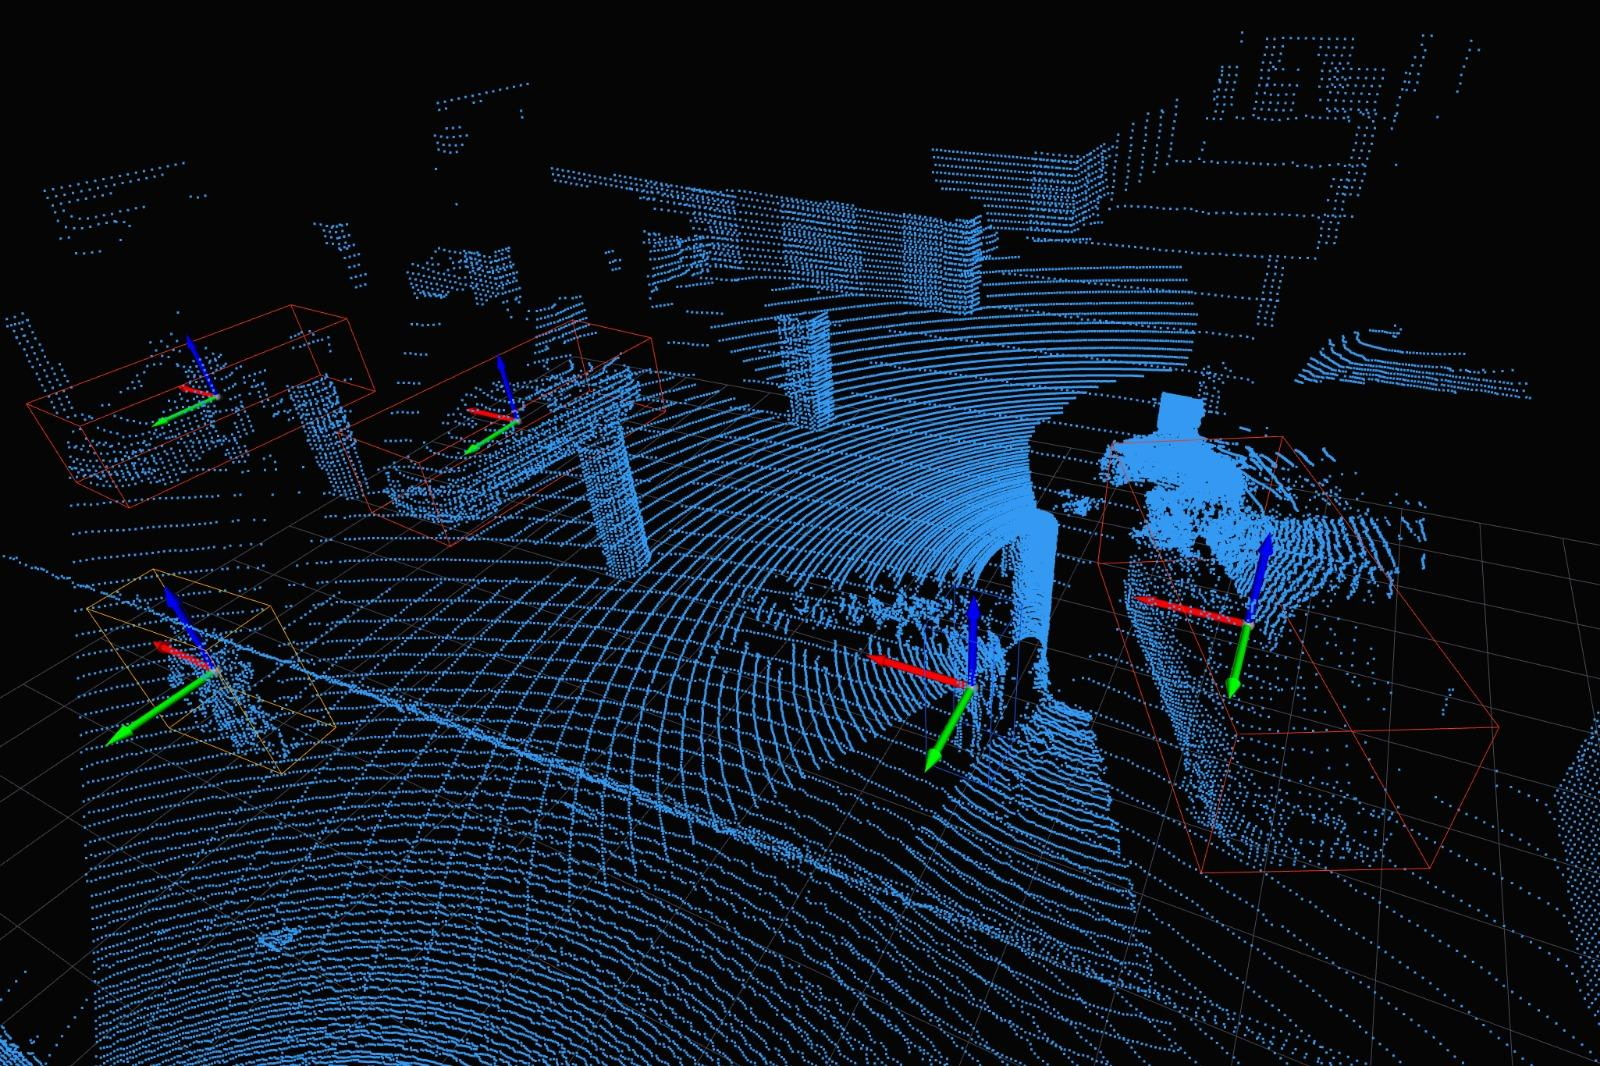
\includegraphics[width=0.95\textwidth]{images/manual-labeling.png}
\caption{Manuelle Nachbearbeitung der Ground-Truth-Annotationen mit dem projektspezifischen Bounding-Box-Editor. Dargestellt ist eine Punktwolke mit orientierten 3D-Boxen für die Klassen Person, Fahrrad und Auto.}
\label{fig:manual-labeling}
\end{figure}

Die ansichtsspezifischen Annotationen sind für den regulären Betrieb sinnvoll, begrenzen aber einen direkten Klassenvergleich zwischen den Ansichten. Beim bewegten Auto ist die Vergleichsmenge exakt gepaart (\(n=339\) in jeder Ansicht). Bei Person und Fahrrad unterscheiden sich die GT-Zahlen. Beispielsweise enthält die gepoolte Fahrradauswertung 718 Instanzen für \texttt{merged}, 627 für \texttt{os0} und 581 für \texttt{os1}.

Diese Differenz ist besonders wichtig für die Interpretation des Fahrrad-AP\textsubscript{30}: \texttt{os0} wird teilweise nur auf dem kürzeren, gut sichtbaren Abschnitt einer Trajektorie bewertet, während \texttt{merged} durch die größere Abdeckung zusätzliche und weiter entfernte Objektpositionen enthält. Der AP\textsubscript{30}-Vorsprung von \texttt{os0} darf deshalb nicht ohne Einschränkung als grundsätzliche Überlegenheit eines Einzelsensors interpretiert werden.
